\chapter{Revisão de Literatura}
\label{ch:fund}


\section{A reprodutibilidade da pesquisa científica}
\label{sec:reprod}

A confiabilidade e a reprodutibilidade são pilares da pesquisa científica moderna, garantindo que os resultados produzidos possam promover o avanço do conhecimento. O método científico na ciência moderna, criada por Francis Bacon, postula que devemos formular uma hipótese, desenhar experimentos para confirmá-la ou refutá-la, analisar os resultados de maneira imparcial, inserir esses resultados no contexto do conhecimento atual e reproduzir esses experimentos.

Entretanto a comunidade científica já identificou e assumiu, em artigos em revistas especializadas, que pesquisadores têm dificuldade em reproduzir experimentos de outros pesquisadores. Principalmente depois que as empresas farmacêuticas Bayer e Amgen terem reportado não poder reproduzir grande parte dos artigos que descrevem drogas como potenciais novos fármacos para o tratamento de câncer e outras doenças.

%https://blog.scielo.org/blog/2017/02/08/avaliacao-sobre-a-reprodutibilidade-de-resultados-de-pesquisa-traz-mais-perguntas-que-respostas
%https://blog.scielo.org/blog/2016/03/31/reprodutibilidade-em-resultados-de-pesquisa-os-desafios-da-atribuicao-de-confiabilidade
%https://blog.scielo.org/blog/2013/07/31/artigo-propoe-quatro-pilares-para-a-comunicacao-cientifica-para-favorecer-a-velocidade-e-a-qualidade-da-ciencia
%http://www2.fesbe.org.br/reprodutibilidade-na-ciencia-uma-noticia-ruim-e-varias-boas/

Iniciativas de reprodutibilidade começaram a surgir em agências de divulgação científica como a \ew{Science Exchange}, que desenvolveu em 2013 a \ew{"Reproducibility Project: Cancer Biology"}, com objetivo de validar 50 artigos publicados entre os mais relevantes e de alto impacto na pesquisa oncológica e \ew{"Reproducibility Project: Psychology"} com a proposta de avaliar a reprodutibilidade de 100 artigos de pesquisa em psicologia, iniciado em 2011 e concluído em 2015, e movido por denúncias de fraude e análise estatística falha em estudos clássicos de psicologia.


Uma pesquisa online realizada pela \ew{Nature} com mais de 1.500 pesquisadores de todas as áreas do conhecimento e publicada em 2016 relevou que mais de 70\% não teve sucesso ao tentar reproduzir experimentos de terceiros e mais de 50\% não pode reproduzir seus próprios experimentos. No entanto, apenas 20\% dos entrevistados afirmam ter sido contatados por outros pesquisadores que não puderam reproduzir seus resultados. Este tópico, entretanto, é delicado, pois corre-se o risco de parecer incompetente ou acusatório. Pelo contrário, quando um resultado não pode ser reproduzido, a tendência dos cientistas é assumir que existe uma razão perfeitamente plausível para o insucesso. De fato, 73\% dos entrevistados são de opinião que ao menos 50\% dos resultados em suas áreas são reprodutíveis, sendo os físicos e químicos entre os mais confiantes. (rescrever)

Quanto à causa da irreprodutibilidade, os fatores mais comuns estão relacionados com a intensa competição e pressão por publicar. Entre os motivos mais citados pelos pesquisadores estão: publicação seletiva de resultados; pressão por publicar; baixa significância estatística; número insuficiente de repetições no próprio laboratório; supervisão insuficiente; metodologia indisponível; design experimental inadequado; dados-fonte indisponíveis; fraude; e avaliação por pares insuficiente.


\section{Fontes de dados}

%https://publicient.hypotheses.org/525
%https://publicient.hypotheses.org/425
%https://blog.scielo.org/blog/2014/07/14/movimento-open-data-se-consolida-internacionalmente/#.W4F5wq1jucM
%https://www.google.com/search?client=firefox-b-ab&ei=SlGBW4vME4T7wQShrbzQCw&q=datasets+para+pesquisa+cient%C3%ADfica&oq=datasets+para+pesquisa+cient%C3%ADfica&gs_l=psy-ab.3...25338.27160.0.28160.0.0.0.0.0.0.0.0..0.0....0...1.1.64.psy-ab..0.0.0....0.vo-Mgdfl8qo


Em artigos científicos tradicionais os dados são vistos como um apoio para as conclusões do artigo de pesquisa, em publicações de dados principalmente em boletins são apresentados novos dados com o objetivo de apoiar novas pesquisas.
A \ew{United States Department of Agriculture} \sigla{USDA}{\ew{United States Department of Agriculture}} atualiza a comunidade científica frequentemente com publicações dados sobre a produção, fornecimento e distribuição agrícola mundial e 11 dos 20 artigos mais citados das revista \ew{Bulletin of the American Meteorological Society} são sobre dados.

Para muitos jornais esse tipo de \ew{data paper} recebe a mesma avaliação do que os outros artigos de pesquisa, sem instruções especificas. Outros jornais possuem instruções sobre a disponibilização dos dados para avaliação por cientistas, porém alguns barreiras como a falta de colaboradores e a avaliação de dados por pares ainda com definições não tão claras, criam uma realidade diferente da esperada. 

A preocupação de manter a publicação permanente dos dados e o vinculo com artigos que os citam, incentivam a parcerias entre bibliotecas e jornais com ferramenta de repositórios de dados (por exemplo http://rda.ucar.edu), de \ew{persistente identifier} como o \sigla{DOI}{\ew{Digital Object Identifier}} e da homogenização dos metadados. Esses vínculos entre repositórios e jornais estão crescendo rápido e os atores formam uma comunidade de avaliação de dados.

Os repositórios de dados criados para instituições ou por centros nacionais de dados, tem uma avaliação mais técnica do que cientifica. Mas a situação esta evoluindo e alguns repositórios começam a exigir uma avaliação do conjunto de dados antes de publicá-los, como a implantação de um plano de gerenciamento de dados que exponha antes do deposito a qualidade e controle dos dados.

\emph{Data Jornals} como Earth System Science Data (Copernicus), Geoscience, Data Journal (Wiley), e Scientific Data (Nature), são jornais específicos para publicação de \ew{data paper} que descrevem um conjunto de dados, disponibilizado dentro de um repositório, explicando as condições de processamento, a coleção e formato de arquivos.


\subsection{Fontes de dados para pesquisa com imagens}

É comum na área de pesquisa em processamento digital de imagens o estudo de fontes de dados tradicionalmente utilizadas na literatura cientifica, quando se propõe novos métodos de análise, podendo comparar os resultados obtidos com trabalhos anteriores. Com exemplo o projeto MNIST.

O projeto MNIST publicado em 1995 é banco de dados de dígitos manuscritos, disponível em http://yann.lecun.com/exdb/mnist/, possui um conjunto de 70.000 exemplos de dígitos normalizados por tamanho e centralizados em uma imagem de dimensões fixas. É um banco de dados para pesquisadores que querem experimentar técnicas de aprendizado e métodos de reconhecimento de padrões em dados do mundo real, enquanto gastam esforços mínimos em pré-processamento e formatação.

Algumas técnicas de reconhecimento de padrões pro processamento de imagens exigem um elevado numero de amostras. Neste sentido surgem projetos como notMNIST de 2011, com a proposta mais de 500 mil imagens de letras geradas digitalmente em fontes tipográficas diferentes. Este projeto apoia a pesquisas em reconhecimento de textos digitalizados ou \sigla{OCR}{\ew{Optical Character Recognition}} e e reconhecimento de textos para tradução em tempo real usando a câmera de celulares.

\begin{figure}[htb]
	\label{teste}
	\centering
	\begin{minipage}{0.4\textwidth}
		\centering
		\caption{Exemplo MNIST} 
		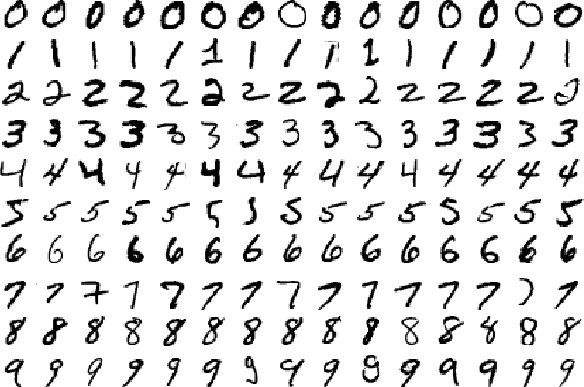
\includegraphics[scale=0.3]{img/mnist.jpeg}
	\end{minipage}
	\hfill
	\begin{minipage}{0.4\textwidth}
		\centering
		\caption{Exemplo notMNIST} 
		
\includegraphics[scale=0.3]{img/nmn.png}
	\end{minipage}
\end{figure}

\begin{figure}[htb]
	\caption{Tradução de textos em imagens}
	\begin{center}
		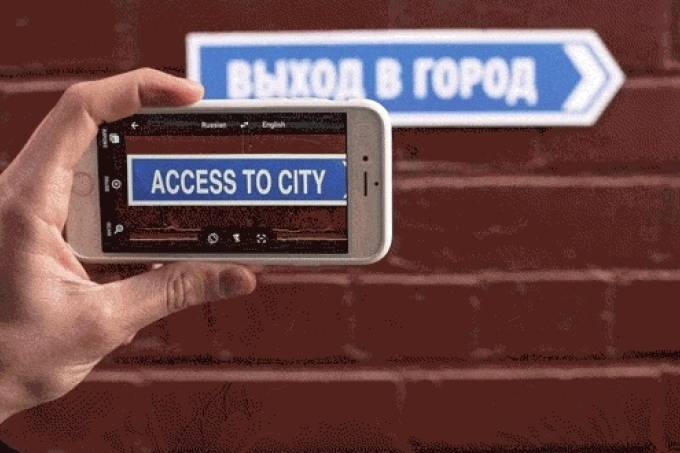
\includegraphics[scale=0.3]{img/google_tradutor.jpeg}
	\end{center}
\end{figure}


O desenvolvimento de bases de imagens para pesquisa são mais comuns no campo da medicina, motivados pelo desenvolvimento de tecnologias de apoio a disgnósticos, como o projeto DMR - Database For Mastology Research (http://visual.ic.uff.br/dmi/) do Instituto de Computação da Universidade Federal Fluminense IC/UFF, que disponibiliza imagens mastológicas térmicas, mamografia, ressonância magnética e de ultrassom para a detecção precoce do câncer de mama.


\subsection{Catalogação de dados}

Quando um pesquisador não tem disponível uma fonte de dados que atenda a área de estudo de seu interesse, este precisa coletar as informações como parte de seu trabalho, para então processá-las e concluir sua pesquisa.

A necessidade de criação de uma base de dados específica, pode exigir uma grande coleta de amostras a campo em uma período curto de tempo, com várias repetições, o que demandaria uma equipe e equipamentos, aumentando o tempo e o custo da pesquisa.

Em um cenário de pouco incentivo em pesquisa e curtos prazos na corrida por publicação, alguns pesquisadores, após investirem na criação de bases de informações adequadas para seus estudos, não facilitam o acesso dos dados para que outros possam pesquisar métodos diferente, fato que poderiam gerar melhores resultados e aumentar o conhecimento científico. Por outro lado, pesquisadores criam projetos que serviram de base para vários outros trabalhos, fomentando a tecnologia e o desenvolvimento do seu campos de pesquisa.

Este trabalho tem a missão de desenvolver uma fonte de dados ampla e confiável, para apoio a pesquisas em uma área importante para o agronegócio brasileiro: a produção de soja.

%a soja%
%A participação do Brasil na Produção Internacional%
%A importância da soja para o mercado financeiro e na indústria alimentícia%
%A importância da soja para o Brasil%
%Sobre o controle de produção%
%Sobre os laboratórios de sementes e os teste%
%Sobre o tetrazólio%


\section{A Soja}
A soja cultivada atualmente é muito diferente dos seus ancestrais, que eram plantas rasteiras que se desenvolviam na costa leste da Ásia, principalmente ao longo do rio Yangtse, na China.  Sua evolução começou com o aparecimento  de plantas oriundas de cruzamentos naturais entre duas espécies de soja selvagem que foram domesticadas e melhoradas por cientistas da antiga China.

Cultivada e consumida há milhares de anos pelas civilizações orientais, foi somente a partir do século vinte que foi comercialmente cultivada no Ocidente, mais precisamente nos Estados Unidos(EUA), a partir da década de 1920. Até 1940, a área de soja cultivada para forragem era maior que a cultivada para grãos. A partir de 1941, a área cultivada para grãos superou a cultivada para forragem. \cite{Amelio2011}

\subsection{A participação do Brasil na Produção Internacional}
Segundo \citeonline{FAS2018}, entre os anos de 19xx e 2017, o Brasil liderou a produção de soja no mundo ao lado dos EUA. Atualmente os dois países juntos são responsáveis por 66\% da produção mundial, com 114,10 e 116,92 milhões de toneladas métricas (mmt). A previsão da produção de soja para 2018/19 no Brasil, por \cite{FAS2018}, é um recorde de 117,0 milhões de toneladas métricas (mmt), em uma área colhida prevista para de 36,5 milhões de hectares (mha), 4\% em relação ao ano anterior, prevendo a produtividade de 3,21 toneladas por hectare, mantendo acima da média dos últimos cinco anos. 

\citeauthor{FAS2018} relata que o Brasil deverá continuar sendo o principal exportador de soja em 2018/19, impulsionados pela forte demanda global liderada pela China por alimentos proteicos, estimulando o esmagamento para obtenção do farelo o óleo de soja.

%ver \cite{Junior2017}

\subsection{A importância da soja para o mercado financeiro e na indústria alimentícia}
A commoditie de soja é negociada nas principais bolsas mundias e seu volume de negociações atualmente segundo (????) é de xxx bilhões de toneladas e yyy bilhões de dólares.\nota{Se este paragrafo for se manter, vou procurar os dados e fontes corretas} No Brasil e em vários países o valor da soja é usado para indexar contratos de diversas naturezas envolvendo o agronegócio, principalmente na compra de terras, maquinários agrícolas e empréstimos para financiamento da produção.

O grão de soja tem grande valor na economia global devido suas propriedades nutricionais e na produção de óleos
Usado na alimentação humana e animal a soja fornece grande quantidade de carboidratos e vitaminas, a proteína de soja é muito usada na indústria alimentícia e gastronômica como alternativa a proteína da carne e do leite, atendendo o mercado vegano e de restrições alimentares. A maior utilização da fibra alimentar da soja é na farinha de soja usada em raça animal, muito utilizada na produção de proteína animal, como carne bovina, suína e de frango.

O processo de beneficiamento da soja inclui a extração do óleo vegetal de soja, largamente usado na indústria alimentícia, sendo um dos mais acessíveis para o consumidor final. Segundo \cite{FAS2018a} o óleo de soja é o mais produzido e consumido no mundo entre as oleaginosas. 

\subsection{A importância da soja para o Brasil}
Para atingir tais grandezas de produção a cadeia agroindustrial da soja emprega certa de XXX pessoas no Brasil, e cerca de YYY empresas recolhendo aproximadamente XXX Milhões de reais em impostos, que representou zz\% da arrecadação do setor primário em 2017.\nota{Se este paragrafo for se manter, vou procurar os dados e fontes corretas}

O cultivo da soja no Brasil ao longo dos anos proporcionou a colonização de regiões pouco habitadas no interior do país, promovendo urbanização e crescimento econômico mais distribuído no território nacional. Entretanto cria um desafio para os produtores de soja, que encontram diferentes climas, biomas, solo, ciclos de chuvas e outros fatores, em um país de proporções continentais. Atualmente o Brasil possui registradas xxx cultivares diferentes de soja, sendo zz transgênicas cada cultivar tem suas características como variando a duração das etapas de produção, produção de óleo ou massa seca, quantidade e tamanho dos grãos, estrutura das plantas (tamanho da planta, raízes, volume de folhas), resistência a seca ou ao excesso de água, resistência a herbicidas, muitas variedades transgênicas são modificadas geneticamente para serem nocivas a determinados predadores, diminuindo o uso de inseticidas e fungicidas. Muita da tecnologia brasileira em sementes se origina da EMBRAPA, que atualmente possuem patentes de xxx cultivares de soja transgênica e zzz patentes de cruzamentos naturais.

ver \cite{Junior2017} \cite{LIMA2013} \nota{Material que comecei a ler e posso usar para embasar o texto}

\subsection{Sobre o controle de produção}
Devido a grande importância que a soja representa para nação brasileira é necessário que se proteja o processo de cultivo. Para isso o estado exige uma série de registros e controles sobre a produção, colheita, comercialização, transporte e exportação. Em cada etapa do processo produtivo da soja existem mecanismos de fiscalização por órgãos competentes.
A legislação Brasileira regula quais variedades de soja tem o cultivo permitido no Brasil, com o intuito de controlar a entrada de plantas que podem ser portas de entrada para fungos e insetos, que podem desequilibrar o ecossistema onde local. Situações como esta já aconteceram no Brasil em culturas de cacau, café e banana no passado, prejudicando a economia e o meio ambiente por vários anos

Para garantir autonomia e proteção dos custos de produção, os produtores de soja no Brasil podem produzir suas próprias sementes para safras futuras, mas se houver comercialização de sementes várias normas de qualidade devem ser seguidas, como por exemplo o teste de germinação que determina que se um lote de sementes não possuir o potencial de germinação mais que 70\% das sementes o lote é inviável para o plantio e deverá ser comercializado como grão no mercado secundário.

??? indica que uma produção inferior a 70\% de germinação é inviável em relação aos custos de produção, desta forma a utilização de lotes controlados aumentam as chances de sucesso na safra, diminuindo os riscos que as financiadoras de crédito e seguradoras rurais têm ao liberarem empréstimos aos produtores. Em 2017 xxx Milhões de reais foram liberados para produção de xx\%v das lavouras na Brasil.

\subsection{Sobre os laboratórios de sementes e os testes}
Até 2017 o Brasil possuem cerca de xx mil empresas e cooperativas que comercializam sementes de soja, sendo que xx\% possuem seus próprios laboratórios de análise de sementes, que realizam diversos testes de rotina, afim de determinar a qualidade e detectar as possíveis causas de problemas, para que estes sejam corrigidos. 

Além dos testes exigidos por lei, os testes oficiais de pureza e germinação, é comum as empresas fazer os testes de qualidade como (patologia  tetrazólio - Vigor - Envelhecimento Acelerado - Teste de emergência em areia - condutividade elétrica), para detectar patógenos e determinar inclusive se o processo de colheita e armazenagem foram feitos com qualidade ou causaram danos nas sementes e comprometeram o lote. Determinar a causa da inviabilidade de um lote é vital para ajustar o processo antes que mais lotes sejam comprometidos.

Os laboratórios de sementes empregam mais de x mil analistas no Brasil inteiro, e todo ano instituições como a EMBRAPA formam novas turmas de analistas para atenderem as demandas do mercado. O investimento que as empresas fazem com laboratório, analistas e equipamentos aumentam o custo da semente, mas agregam muito valor na qualidade e garantia das safras seguintes.

\subsection{Sobre o tetrazólio}
Uma das análises mais importantes de um laboratório de sementes de soja é o teste de \sigla{TZ}{Tetrazólio}, que a partir de uma amostra do lote de sementes, tem o objetivo de ressaltar os danos causados em cada semente, para que seja determinada em primeiro momento a viabilidade do lote e a vigorosidade que as plantas terão ao serem plantadas, e em segundo momento se houverem danos nas sementes, determinar o grau dos danos e as causas, que geralmente são causados por excesso de umidade no armazenamento, danos mecânicos do processo de colheita, secagem e estocagem; e danos causados por percevejos que se alimentam dos nutrientes contidos nas sementes.

Para realização do teste cada amostra é submetida a uma solução de sal de tetrazólio por até x horas, dependendo da metodologia usada, durante esta etapa a semente absorve a solução ficando maior e destacando em tons de vermelho carmim os danos que cada semente sofreu. Após a preparação inicial, cada semente é cortada no sentido transversal a radícula para análise do interior e exterior da mesma, na sequência é realizada uma minuciosa analise visual de cada metade da semente em busca de padrões característicos dos danos mencionados, os danos de cada semente são anotados em uma ficha de controle e ao final o analista calcula os resultados que classificam o lote.

As limitações do teste de tetrazólio, citadas por FRANÇA-NETO (1998) incluem a exigência de um treinamento especial sobre a estrutura embrionária da semente, experiência e paciência pois a análise é relativamente tediosa. Atualmente o mercado exige cada vez mais profissionais capacitados em realizar o teste.


Dada a importância que o teste de tetrazólio tem no processo de garantia de sucesso no cultivo da soja, e a importância da cadeia produtiva no Brasil e no mundo, é justificável que pesquisas sejam aplicadas com o objetivo de tornar o processo de análise mais rápido e assertivo.



%\section{Sobre o projeto}


%openCV android




\section{Flutter}


%%%%%%%%%%%%%%%%%%%

%%%%%%%%%%%%%%%%%%%

Eu vou estar indo sobre o b�sico de Dart, especialmente porque � usado por flutter e mais desenvolvimento de aplicativos ganhou muita tra��o ao longo dos anos e h� um monte de lucro a ser ganho.


Eu come�o falando sobre flutter e depois me movo para o dardo.



2. O que � Flutter?

Vamos come�ar com o primeiro take o que � flirter para aqueles de voc�s que talvez n�o conhe�am o Google Flirter como o nome indica � SDK de aplicativo m�vel do Google, que pode ser usado para criar interfaces nativas de alta qualidade em iOS e Android em um curto per�odo de tempo.

O lan�amento inicial do flirter foi em maio de 2017.

Tamb�m uma nota lateral SDK significa desenvolvimento de software.

Boa.

Voc� deve saber que o flirter faz uso do c�digo existente para funcionar.

Os muitos benef�cios oferecidos o levaram a ser usado por desenvolvedores de aplicativos independentes e at� por organiza��es famosas em todo o mundo.

Tamb�m � livre para usar uma fonte aberta.

Algumas das coisas b�sicas sobre o flerte que voc� deve tomar nota.

Nosso n�mero um desenvolvimento r�pido usando flirter.

Voc� pode ter recarregado em uma quantidade de milissegundos para garantir que seu aplicativo possa ganhar vida no menor tempo poss�vel.

Voc� tamb�m pode usar uma vasta gama de widgets totalmente personaliz�veis ??que ajudam a criar interfaces nativas da maneira mais r�pida poss�vel.

Eu estou falando de ser capaz de construir em minutos aqui.

N�mero dois interface expressiva e flex�vel s�o interface do usu�rio.

Seu aplicativo n�o pode ser bem-sucedido se n�o for f�cil de usar para as pessoas.

Os melhores aplicativos l� fora tamb�m apresentavam a melhor experi�ncia e a experi�ncia do usu�rio.

Ent�o, o que voc� conseguir mais ferramentas para garantir que o nativo e experi�ncia do usu�rio � o melhor que pode ser.

A arquitetura em camadas oferece acesso � personaliza��o completa, permitindo que voc� crie aplicativos interativos e amig�veis ??ao usu�rio, que t�m uma renderiza��o de renderiza��o incrivelmente r�pida, al�m de um expressivo desempenho nativo da �rvore de n�meros.

Independentemente de uma pessoa estar usando um dispositivo Android e iOS, seu aplicativo precisa oferecer a experi�ncia que eles esperam que os widgets no flertador possam incorporar todas as diferen�as cr�ticas de plataforma para garantir a qualidade.

Essas diferen�as negras incluem �cones de rolagem de navega��o e garfos para a incorpora��o do DS �s diferen�as. O desempenho nativo de seus aplicativos em dispositivos Android e iOS � mantido no n�vel ideal.

Agora que voc� adquiriu um conhecimento b�sico do Google Flirter, deixe-me dar uma r�pida introdu��o indireta ao escuro.



3 O que � o Dart?

O que � obscuro quando se trata de entender darte voc� deve saber que j� � um objeto e fez e florescer a linguagem definida que voc� usa a sintaxe no estilo C que compila opcionalmente no javascript d'arte oferece muito apoio.

Isso significa que ele pode suportar interfaces de classes abstratas que fazem sentido digita��o est�tica e at� mesmo um sistema de tipo de som.

Agora, todos esses termos podem soar um pouco demais para aqueles que n�o est�o familiarizados com esse jarg�o.

Bem, deixe-me tornar as coisas mais f�ceis para voc�.

Basicamente escuro ajuda voc� a criar lindas experi�ncias de alta qualidade em todas as telas de dispositivos por meio de uma linguagem que nega a otimiza��o de ferramentas flex�veis f�ceis de usar e de estruturas muito poderosas e ricas no pr�ximo cap�tulo.

Falarei sobre e levarei todos voc�s em um breve hist�rico de desenvolvimento de aplicativos para dispositivos m�veis, como evolu�ram ao longo dos tempos e por que voc�, como um poss�vel desenvolvedor da ABB, pode se tornar conhecido nesse campo por meio do Google furter ou talvez de algum outro SDK voc� est� confort�vel com o uso.

Ent�o vamos seguir em frente.


Se��o 2: A Hist�ria do Desenvolvimento de Aplicativos M�veis

4. Conhecendo seu hist�rico de aplicativos

Como mencionei, o desenvolvimento de aplicativos cresceu muito nos �ltimos anos.

Como algu�m que est� interessado em entrar nesse campo, ser� bom ter uma vis�o geral de como o mercado de desenvolvimento de aplicativos para dispositivos m�veis cresceu.

Quando eles foram introduzidos pela primeira vez, os telefones celulares foram completados como tecnologia que era usada apenas para fazer liga��es telef�nicas.

No entanto, mais tarde, como sabemos que o jogo mudar a inven��o de smartphones levou � abertura da porta de desenvolvimento de aplicativos m�veis, os aplicativos de software s�o como os chamamos de trabalho para lev�-los a executar ou operar em dispositivos m�veis modernos, como tablets e smartphones.

Com o passar dos anos, esses aplicativos foram aprimorados e agora parece ter se tornado uma parte importante de nossas vidas.

Eles parecem ter se integrado perfeitamente ao nosso estilo de vida, come�ando pelo in�cio do celular.

Vamos come�ar isso de todo o caminho de volta.

Sim, estou falando do come�o do celular e sim da primeira liga��o de celular feita.

Para aqueles de voc�s que n�o conhecem a primeira liga��o de celular j� feita, em 3 de abril de 1973, a mesma liga��o foi feita por Martin Cooper, da Motorola.

De fato, esse telefonema era basicamente um golpe de publicidade para a grande empresa.

N�o foi at� 10 anos depois, desde que a bola que o primeiro telefone celular atingiu oficialmente o mercado, mesmo assim, o jornal p�blico n�o foi capaz de us�-lo.

Por qu�.

Bem, porque a morte n�o � o primeiro telefone celular no mercado custou uma grana por \$ 2000 e pesava aproximadamente � 2.

Sim.

Isso � muito.

Agora, � claro, esse modelo inicial da Foon n�o tinha nenhum aplicativo.

Quero dizer, as pessoas provavelmente nem sabiam sobre apps naquela �poca, foi na d�cada de 1990, quando o BBH foi introduzido como os primeiros sistemas operacionais que permitiam aplicativos durante esse tempo espec�fico.

Esses dispositivos eram aqueles que inclu�am processadores de texto e bancos de dados de planilhas do di�rio.

� claro que a tecnologia melhorou e o TAAS BDA � um trabalho para se tornar acess�vel ao lidar com mais aplicativos.

Era uma linguagem de programa��o aberta que possibilitava aos usu�rios criar seus pr�prios aplicativos para o desenvolvimento de aplicativos personalizados.

As empresas precisam de dispositivos Foster e sim de sistemas operacionais ainda melhores.

Voc� pode n�o perceber isso agora, mas o lan�amento do smartphone BlackBerry, que n�o chegou l� em 2002, foi anunciado como uma grande conquista para as empresas de tecnologia.

Esse tipo de telefone foi capaz de integrar perfeitamente o email sem fio e outros recursos que foram os primeiros de muitos durante esse per�odo.

Java m e era muito popular para telefones e Beedi � por isso que voc� pode perguntar.

Isso porque permitia aos usu�rios espa�o adicional na mem�ria.

Ent�o, em 2009, o lan�amento do Symbian abriu as portas para novos desenvolvimentos ainda mais de acordo com os dados, pelo menos, 50 milh�es de dispositivos adotaram o sistema operacional Symbian depois que foi lan�ado.

Mesmo aparelhos da Nokia, aparelhos da Samsung e at� mesmo telefones LG come�aram a usar o novo sistema operacional para melhorar a si mesmos como marcas.

Ent�o, chegando ao desenvolvimento de aplicativos personalizados que atingiram o mainstream Bem, uma vez que os desenvolvedores come�aram o desenvolvimento come�ou a acelerar.

N�o demorou muito para que os apps atingissem o mainstream e o tempo do Grant.

Vivemos no.

N�s basicamente temos um aplicativo para cada tanque.

No entanto, voltando � hist�ria de tudo em 2007, o primeiro iPhone foi lan�ado pela Apple, a App Store foi adicionado pela empresa muito em seguida, permitindo aos usu�rios encontrar baixar e usar aplicativos.

No come�o, esses aplicativos eram limitados, mas n�o demorou muito para que os desenvolvedores de aplicativos descobrissem o potencial inexplorado nesse campo.

Seguindo o exemplo, o mercado Android deu �s pessoas uma outra plataforma para acessar aplicativos e at� hoje h� uma competi��o entre o aplicativo da Apple e do Android e eu acho que � para continuar.

E enquanto a competi��o entre o Android e a Apple continua e os desenvolvedores olham para as plataformas planas da base de clientes potenciais, forne�a-as.


Se��o 3: Por que usar o Flutter?
5. Entendendo por que voc� deve considerar o uso do Google
Flutter


Duvido que voc� conhe�a um pouco mais sobre o slurper e como ele pode ajudar voc� como desenvolvedor de aplicativos.

Vamos ver porque voc� deveria usar o Slichter.

Como mencionado antes, o flirter � o K Isso significa um kit de desenvolvimento de software.

� considerado por muitos como uma maneira eficiente de criar aplicativos m�veis de plataforma cruzada com uma interface de usu�rio ou interface do usu�rio impressionante.

Observe que a maneira desordenada de criar visualiza��es tem semelhan�as com o aplicativo da web.

� a� que voc� pode encontrar v�rias analogias para DML e CFS.

De acordo com os desenvolvedores do selector schlechter torna mais f�cil e r�pido para construir um belo aplicativo m�vel D-Wave flicker para a maioria das c�lulas.

Parece bom.

No entanto, para aqueles de voc�s que talvez n�o saibam sobre outras solu��es de plataforma cruzada, como Zahm nativo de re-a��o i�nica, voc� pode querer saber um pouco mais sobre como o Slichter pode ajudar.

Existem certos benef�cios ou o flerte Stec pode ajud�-lo a mudar de ideia.

E voc� sabe que voc� precisa come�ar a us�-lo.

Alguns de voc�s podem ter muitas perguntas sobre flertes agora.

Como funciona a carta?

Por que � considerado inovador pelos outros?

Por que eles deveriam us�-lo?

Etc ..

E espero responder a todos eles no discurso.

E embarque no benef�cio de o flicker ser o SDK im�vel para a cria��o de aplicativos m�veis de plataforma cruzada Krok � que voc� pode escrever um c�digo e depois executar o aplicativo no iOS e no Android.

O c�digo que voc� escreve tem que ser escrito no escuro.

Ent�o, qualquer idioma desenvolvido pelo Google Docs parecer� familiar para voc�.

Se voc� j� teve experi�ncia de usar Java antes.

Tome nota que, em vez de usar arquivos SML, voc� constr�i um layout.

Tal lay out � constru�do a partir de componentes de widgets que s�o aninhados seu widget � um aplicativo de material que � o aplicativo inteiro e, em seguida, voc� tem desconforto que � Dumaine lay out estrutura, em seguida, movendo-se dentro.

Voc� tem a barra de aplicativos que � como a barra de ferramentas do Android 2 e, em seguida, um cont�iner como o corpo.

Agora, � nesse corpo que voc� coloca os widgets layouts, como bot�es, texto, etc., avan�ando ou por que voc� deve considerar o uso do clicker. Veja uma lista.

N�mero um de recarga quente.

Como mencionado antes, o recarregamento do Hawks pode ser considerado como outro melhor recurso que � usado para recarregar.

Voc� pode criar instantaneamente os projetos em que est� trabalhando, como se estivesse construindo uma p�gina da Web, simplesmente alterando algo no c�digo.

Clique em carga de Hawtry e voc� poder� ver o resultado instantaneamente.

N�mero dois um conjunto inteiro de widgets de design de material que flertam voc� come�a a obter a ecosfera registrada com constru�do em componentes de interface do usu�rio, voc� deve tomar nota de que existem dois conjuntos de rejei��es.

H� o design do material que � para o Android e o Cupertino do Derrida, que � para iOS.

Voc� simplesmente tem que selecionar o widget que voc� quer e depois ir a partir da�.

Tamb�m n�o h� necessidade de voc� se preocupar com o fato de os widgets serem muito espec�ficos.

Isso significa que, mesmo que voc� acabe implementando alguns Cupertino, os widgets projetados por Maduna v�o acabar parecendo iguais em todos os dispositivos iOS e Android existentes.

Portanto, n�o h� necessidade de voc� se preocupar com algo em seu aplicativo ou at� mesmo com o aplicativo como um todo, parecendo diferente.

Quando executado em dispositivos diferentes No entanto, voc� pode usar diferentes equipes Android e iOS, se desejar.

Tamb�m tudo � um widget em flertar.

Sim, at� mesmo a sua classe de aplicativo, o aplicativo de material � um widget.

Ent�o, toda a sua estrutura de layouts � escaneada por dimens�o.

Ent�o, ter tudo como um widget permite que voc� use flirter para criar UI impressionante de uma maneira muito simples.

Numero tres.

V�rios pacotes, apesar de terem sido lan�ados mortos.

Recentemente, em 2007, a comunidade deflectiva de Dean � muito ativa e envolvida em torn�-la melhor.

Isso fez com que o flatter fosse capaz de suportar muitos pacotes que voc� tem acesso a pacotes para abrir imagens compartilhando a corrente e fazer solicita��es de HDTV acessando sensores armazenando suas prefer�ncias.

Implementando Firebase e a lista continua.

Todo esse suporte � para iOS e Android.

Agora que voc� passou por cima dos benef�cios do sluttier, pergunte a si mesmo. Voc� est� interessado em usar o flirter?

N�o h� necessidade de tomar uma decis�o precipitada.

Estarei falando mais sobre tudo isso enquanto o discurso continua.


Se��o 4: Como instalar o Flutter?
6. Instalando o Flutter para Windows, Linux e MacOS

N�mero um dos seus sistemas operacionais deve ser o Windows 7 S-B 1 s�o mais tarde de 64 bits, voc� precisa de pelo menos 400 M-B ou tr�s espa�o em disco.

Tome nota que n�o inclui este lugar para Dools.

Falando sobre as ferramentas que voc� precisa.

Ponto de shellfire Bovver.

Ou voc� n�o precisa.

Este � o G ID para o Windows.

Quando eles usam boa op��o de prompt de comando do Windows.

Se voc� tiver para o Windows j� est� instalado.

Precisa ter certeza de que voc� pode executar o comando get para o prompt de comando ou instalar o flirter no Mac

SO para instalar e executar o flirter no Mac OS, seu ambiente de desenvolvimento deve atender a esses requisitos m�nimos.

Estes s�o o sistema operacional deve ser, pelo menos, Mac OS 64 bits, pelo menos, 700 M-B de espa�o livre em disco.

Novamente, isso n�o inclui espa�o em disco para Dools.

Agora, observe que o flertador depende de v�rias ferramentas de linha de comando dispon�veis em seu ambiente.

Estes s�o Bash e Diyar r m.

Boa menina.

Descompacte e at� mesmo a �rvore num�rica.

Continuando a instalar o flirter no Linux para instalar e executar o flirter no Linux.

Voc� precisa de um sistema operacional que seja o Linux 64 bit 600 M-B de espa�o livre em disco.

Isso n�o inclui espa�o em disco para o seletor Dools, dependendo de algumas ferramentas de linha de comando dispon�veis

em seu ambiente.

Estes s�o novamente Bash e ganham Diyar.

R m.

Boa menina.

Descompacte e qual comando de teste flexor depende da biblioteca estar dispon�vel em seu ambiente que

� como voc� pode ver lib G.O. voc� Daut s o dot um fornecido por mim de bagagem, por exemplo l AB lib Glou one me no Ubuntu s�o Debian.

Voc� pode v�-lo no slide, ent�o n�o deixe de reservar o site oficial do seletor.

Voc� tem uma ideia mais aprofundada sobre o procedimento que precisa ser seguido para instalar e come�ar a usar o flexor.



Se��o 5: Benef�cios do Flutter
7. Benef�cios do Flutter

Com base em uma parte do Curso onde eu falei sobre o motivo pelo qual voc� deve considerar o uso do flirter um pouco mais sobre todos os benef�cios e pode oferecer a voc� muitos desenvolvedores recomendam usar o flirter.

Se voc� est� apenas come�ando no campo de desenvolvimento de aplicativos por causa de sua natureza amig�vel quando se trata de criar aplicativos multiplataforma, vamos passar por cima de uma lista.

Flirter de projeto de c�digo aberto n�mero um � um projeto de c�digo aberto que permite que ele esteja dispon�vel para uso tamb�m por startups.

Ele oferece muitas op��es para criar o tipo de aplicativo que voc� deseja criar para Android ou iOS.

Al�m disso, sendo de c�digo aberto, d� origem � colabora��o aberta, permitindo que outros ajudem a melhorar ou fa�a o n�mero dois de Ed impressionantes. integra��o usando flirter.

Voc� pode continuar e continuar adicionando e subtraindo edi��es durante o processo de desenvolvimento do aplicativo.

Oferece uma impressionante integra��o de edi��o com o est�dio Android e o c�digo do Visual Studio.

Isso leva a conclus�es mais inteligentes baseadas em onde os tipos de defini��es usuais e o n�mero de m�dulos importados criam campos escuros como o Java.

Por que a dieta diet�tica n�o � uma c�pia direta do Java.

Os dois s�o semelhantes a similaridades.

Ajude os desenvolvedores a mudar para o escuro.

Se eles est�o usando Java para o n�mero quatro da lista, temos 4 gerentes de engenharia que gerentes de engenharia tamb�m podem usar o flirter se tiverem a necessidade de liderar mais equipes de desenvolvimento biol�gico usando um SDK como gerente de engenharia.

Voc� pode criar uma equipe surda de um �nico aplicativo m�vel ou uma equipe de desenvolvimento para ajudar voc� a unificar os investimentos em desenvolvimento.

Voc� pode enviar recursos mais rapidamente para reduzir seus custos de manuten��o e transferir os mesmos recursos para o Android e o iOS simultaneamente.

Em suma, quando voc� est� usando a desordem, voc� tem acesso a melhores recursos de widgets f�ceis de usar e integra��es editoriais impressionantes para o desenvolvimento de aplicativos.

N�o � de admirar que muitos desenvolvedores tenham usado o seletor para criar aplicativos m�veis, mas tamb�m para alcan�ar um p�blico mais amplo.

No Android e no iOS.

Se��o 6: Quanta Experi�ncia como Desenvolvedor de Aplicativos
Devo ter que usar o Flutter?

8. Quanta experi�ncia como desenvolvedor de aplicativos eu deveria
tem que usar o Flutter?

Esta � a pergunta que muitos de voc�s podem ter atualmente.

Em suma, voc� n�o precisa de nenhuma experi�ncia anterior para aprender e usar flirter.

Este SDK � muito acess�vel para programadores que t�m uma ideia sobre conceitos de programa��o imperativa e conceitos orientados a objetos.

Contanto que voc� tenha paix�o e interesse em usar a desordem para criar aplicativos, voc� achar� o processo bastante f�cil e r�pido.

Vamos falar sobre isso um pouco mais.

N�mero um do estilo reativo ao usar o flirter, voc� precisar� come�ar em algum lugar para criar um aplicativo para iOS e Android.

� por isso que voc� precisa estar pronto para trabalhar usando uma estrutura reativa.

N�mero fazer.

David voc� n�o pode falar sobre seletor sem falar sobre a arquitetura de widgets que oferece.

Como mencionado tudo � o widget e seletor de seu elemento de estrutura para eles e voc� � o bot�o dois elemento muito estil�stico que voc� deseja usar, como um esquema de cores e formatar tudo.

� um isolante r�gido que permite criar o tipo de aplicativo que voc� quer sem problemas.

Voc� ganha muito controle sobre a renderiza��o do objeto de composi��o de execu��o do aplicativo e mais n�mero tr�s.

Diga adeus ao gerenciamento do ciclo de vida da atividade.

Se voc� � algu�m que se envolveu um pouco no desenvolvimento de aplicativos, voc� estar� familiarizado com o gerenciamento do ciclo de vida da atividade.

Ele s� aparece como trabalho extra, n�o �?

Uma atividade perif�rica, se poss�vel, que n�o seja adicionada diretamente no processo geral de produ��o de seu aplicativo.

No entanto, o que flertar voc� n�o ter� que se preocupar com o gerenciamento do ciclo de vida da atividade.

Isso ocorre porque o patch do conector de desordem ajuda a fazer com que todas as atividades transmitidas sejam vestidas e carregadas de maneira s�ncrona.

N�mero de 60 SPSS consistentes s�o quadros por segundo.

O Flirter tamb�m � �til para quem procura criar um seletor de aplicativos gr�ficos ou de jogos pesados, capaz de oferecer uma taxa consistente de 60 quadros por segundo devido � natureza reativa e ao uso de suporte sombrio.

Voc� ter� visuais est�veis ??em seu aplicativo desenvolvido.

O n�mero cinco, o flertador de suporte da comunidade, tamb�m tem uma grande comunidade de expedientes, al�m de demitir desenvolvedores que podem ajud�-lo com o suporte necess�rio que voc� precisa.

A comunidade torna mais f�cil para voc� aprender usando o flerte, bem como fazer conex�es �teis no campo de desenvolvimento de aplicativos.

Ent�o, vamos falar um pouco sobre darte e por que Slichter usa o come�o.

Se��o 7: Conhecendo o Dart
9. O que � o Dart e por que us�-lo?

Durante este curso eu mencionei d'arte muito como uma pequena atualiza��o.

Dart � uma linguagem de programa��o de uso geral que foi originalmente desenvolvida pelo Google.

Mais tarde foi aprovado como padr�o pela ECMA daks ECMA para 8 para ser mais preciso.

Voc� pode usar d'arte para construir aplica��es web e m�veis para servidores.

Ent�o, por que os desenvolvedores do d'arte trabalham no Google, al�m de outros.

N�o use darte para criar aplicativos de alta qualidade para iOS.

E Android, assim como a web.

Ent�o � por isso que pode ser visto ou � visto como uma �tima op��o quando se trabalha com recursos voltados para o desenvolvimento do lado do cliente.

Vamos a uma lista sobre o Bart.

A sintaxe escura produtiva n�mero um � clara e concisa.

O ferramental geral � muito simples, mas poderoso.

Voc� pode identificar erros sutis precocemente atrav�s da digita��o de sons usando darte.

Voc� tamb�m pode obter in�meras bibliotecas de pontua��o e milhares de pacotes.

N�mero dois r�pido Dart pode ser denominado como uma linguagem que oferece otimiza��o antes da viola��o.

Isso ajuda voc� a obter desempenho previsivelmente alto e inicializa��o r�pida em dispositivos m�veis e na Web.

O n�mero tr�s vi�vel para aplicativos m�veis escuros � executado de forma nativa no Android e no iOS.

Compiladores sombrios fazem A-R como um c�digo X 86.

Tome nota DEC para web app caiu spiles para javascript e � acess�vel.

Muitos desenvolvedores est�o familiarizados com o d'arte que voc� faz.

N�o � uma orienta��o e sintaxe de objeto sem surpresas.

Voc� pode facilmente pegar o jeito escuro se voc� j� sabe sobre Java s�o C ++.

Agora, se voc� sabe um pouco mais sobre d'arte Lexi, por que voc� deve considerar aprend�-lo em 2018, bem como por que o flerte faz uso do efeito.

Se��o 8: Por que voc� deve considerar o aprendizado de dardo em
2018

10. Se voc� considerar a aprendizagem do dardo em 2018 e
Al�m?

Se voc� tem pensado em aprender, aqui est� uma lista que pode ajud�-lo a tomar uma decis�o.

N�mero um f�cil de aprender.

Como mencionado anteriormente, os guardas de Daryn compartilham semelhan�as com outras linguagens comuns.

Isso tamb�m significa que voc� j� deve saber como usar d'arte sem perceber que ser� f�cil para voc� aprender se tiver experi�ncia com outras linguagens orientadas a objetos, como Java, s�o C ++.

Mesmo se voc� souber alguma aprendizagem sobre javascript, Darb n�o ser� dif�cil para voc�.

Outra grande coisa � que o dardo suporta tanto a digita��o solta quanto a forte.

Isso permite que seja mais f�cil quando voc� est� mudando de outro idioma.

Number faz uma base de c�digo compartilhada nativamente compilada.

Alguns de voc�s podem saber que outras estruturas permitem que voc� compartilhe partes da base de c�digo em diferentes plataformas.

No entanto escuro � um pouco diferente.

Ele permite que voc� escreva um �nico aplicativo que pode ser usado tanto no iOS quanto no Android, juntamente com a maneira como ele � compilado nativamente pelo Dubost.

Agora, � claro, isso � algo que os outros podem fazer, mas o darte � capaz de permitir ainda mais o compartilhamento.

Voc� sabe que eu posso dizer que permite que voc� compartilhe um pouco do seu c�digo entre a inteireza do seu GUI, n�o apenas os aplicativos m�veis fazem o Menke para diferentes plataformas, significando iOS e Android, mas tamb�m para a Web, bem como outras aplica��es de guarda tamb�m .

Isso permite que voc� compartilhe a maior parte do c�digo n�o UI ou digamos que o c�digo espec�fico em preto com o n�mero de frameworks do Underdark seja produtivo. Usando o escuro, voc� ter� a experi�ncia de como � f�cil e r�pido criar o layout e adicionar funcionalidade para o seu aplicativo.

Voc� pode criar o Caly no c�digo criando uma s�rie de widgets.

Lembre-se do que eu disse a voc� que, em flertar, tudo o que o widget usa com essas ferramentas certamente ajudar� voc� a criar o que quiser no menor tempo poss�vel.

N�mero quatro compila antes do tempo e apenas no tempo quando voc� est� desenvolvendo um aplicativo Avodart voc� pode ver as mudan�as que voc� faz instantaneamente.

Isso significa que voc� n�o ter� que passar pelo procedimento de recompila��o e n�o h� necessidade de esperar que o aplicativo seja recarregado.

Voc� s� precisa salvar a altera��o e ver instantaneamente as altera��es.

Isso � poss�vel porque, com essa estrutura de desenvolvimento de aplicativo para celular, voc� pode compilar antecipadamente.

R E ou D, bem como na hora certa.

R d.

Agora que voc� est� ciente das raz�es mencionadas, voc� provavelmente est� come�ando a entender o benef�cio de usar o darte.

Experimente e veja se � algo sobre o qual voc� deseja aprender mais.

Como um desenvolvedor de aplicativos que est� mudando meu discurso, eu deixo voc� saber por que flirter escolheu usar d'arte.

Se��o 9: Por que o Flutter usa Dart?

11. Por que o Flutter Decidiu Usar o Dart?
Flirter decidir usar d'arte n�o foi uma decis�o precipitada.

Flirter usa essa ferramenta.

Um total de quatro dimens�es prim�rias para avalia��o e considerou todas as necessidades dos autores, desenvolvedores e usu�rios finais do framework.

Foi fundada enquanto algumas l�nguas cumpriam certos requisitos.

Estava escuro l�.

Marcou muito em todas as dimens�es de avalia��o que foram verificadas pela equipe mais plana e tamb�m atendeu a todos os requisitos e crit�rios determinados.

Voc� deve saber que os dubladores de Darkthrone e compiladores suportam a combina��o de dois recursos cr�ticos para flertar um parding ao tema de flutter.

O primeiro � o ciclo de desenvolvimento r�pido baseado em GAAP, que permite a mudan�a de forma e a carga de Hawtry com estado na linguagem com tipos.

Como eu mencionei anteriormente, o GAAP est� na hora certa.

A segunda � a antecipa��o de nosso descompilador imenso, que emite uma importa��o A-R eficiente para uma inicializa��o r�pida e desempenho previs�vel de implementa��es de produ��o.

Al�m disso, a equipe de flirter foi capaz de trabalhar de perto com a comunidade DAR.

A comunidade � ativa e continua a investir recursos para melhorar o desenho quando se trata de us�-lo como exemplo.

Quando a equipe adotada darte decidiu definhar n�o teve uma hora antes do tempo ou toolbol AOB Freberg usando bin�rio nativo � um tal recurso � fundamental para alcan�ar alto desempenho previs�vel.

No entanto, agora a linguagem tem isso porque eles s�o dark deam e eles est�o construindo para Lucker no dia prim�rio um grande dia com dark marcou uma pontua��o alta para a vibra��o deam foram n�mero um produtividade do desenvolvedor de acordo com o tema.

Uma das principais proposi��es de valor de letras � que ele economiza recursos de engenharia, permitindo que desenvolvedores criem aplicativos para iOS e Android com a mesma base de c�digo usando uma linguagem altamente produtiva que acelera os desenvolvedores Forder e torna a carta mais atraente para eles.

Isso foi muito importante para a equipe de framework defletor da Dubow, bem como para os desenvolvedores.

Voc� deve saber que a maior parte da sorte � constru�da na mesma linguagem dada aos usu�rios.

Portanto, o tema precisa permanecer produtivo em cem mil linhas de c�digo sem sacrificar a acessibilidade ou a legibilidade da estrutura e dos widgets para os desenvolvedores.

Orienta��o n�mero dois objeto para flirter que vorn tema fez uma linguagem que foi adequado para flusters dom�nio do problema que � bom outra coisa que voc� vai usar suas experi�ncias de acordo com a equipe da ind�stria tem v�rias d�cadas de conveni�ncia construindo frameworks de interface do usu�rio em linguagens orientadas a objeto.

Embora eles possam ter usado uma linguagem conhecida orientada a objetos, isso significaria reinventar a roda para resolver v�rios problemas dif�ceis.

Al�m disso, a grande maioria dos desenvolvedores j� tem experi�ncia com desenvolvimento orientado a objetos, tornando mais f�cil aprender como desenvolver seus aplicativos, cujo seletor agora possui um alto desempenho previs�vel de acordo com o refletor de temas.

Eles querem capacitar os desenvolvedores para criar experi�ncias de usu�rio r�pidas e fluidas.

Ent�o, para que eles cumpram essa promessa ou objetivo, eles precisam ser capazes de executar uma quantidade significativa de placa de desenvolvedor durante cada quadro de anima��o.

Isso significa que a equipe precisava de uma linguagem que pudesse fornecer alto desempenho e fornecer desempenho previs�vel sem bater seus chefes.

Isso poderia causar o n�mero de quadros perdidos para localiza��o fasc neste ponto.

Voc� deve saber que a estrutura do defletor utiliza um fluxo de estilo funcional que, de acordo com o tema da letra, depende muito do eficiente alocador de mem�ria subjacente que manipula com efici�ncia o pequeno local de curta dura��o.

Este arquivo foi desenvolvido em linguagens com essa propriedade e n�o funciona de maneira eficiente em idiomas como esse recurso.

Ent�o agora voc� sabe por que flutter decidiu usar d'arte e por que voc� deveria estar familiarizado com tal linguagem.

E quem sabe voc� pode querer us�-lo tamb�m.


Se��o 10: Perguntas Freq�entes sobre o Flutter
12. O que h� dentro do Flutter SDK?
Permita-me ir com freq��ncia para fazer perguntas que voc� possa ter em mente que desapontam.

A primeira pergunta � o que est� dentro do SDK flertador.

Quando se trata de responder o que est� dentro do deflector SDK.

Aqui est� a lista.

O n�mero um otimizou fortemente o primeiro mecanismo de renderiza��o de leads duplo da Mumbai com excelente suporte para texto.

Em seguida, temos o conjunto de widgets de estilo de re-ato de Morgan o conjunto rico de widgets para Android e iOS que eu disse anteriormente tudo � um widget em flertar.

N�mero quatro, � bom para testes de unidade e integra��o.

Em seguida, entramos em interoperabilidade e plug-in API para conectar-se ao sistema e participar D DST gais headless best runner para executar testes em ferramentas de linha de comando do Windows Linux e Mac para criar testes de constru��o e compilar seus aplicativos.

13. O Flutter vem com uma estrutura?

Faz flutter vem com o quadro.

Sim.

Como desenvolvedores de aplicativos, voc� deve saber que os sistemas de terra plana com uma estrutura moderna inspirada pela estrutura de aletas de re-a��o foram projetados para serem lidos e personaliz�veis ??como um desenvolvedor.

Voc� pode ir em frente e optar por usar apenas parte do framework que voc� tem acesso, voc� � um framework completamente diferente.

A escolha � sua.


14. O Flutter vem com widgets?
Faz flutter vem com Vineyard como mencionado antes que sacode no parque e parte de flutter.

Ent�o, sim, selecione seus navios com um conjunto de alta qualidade McKeel design em layouts e equipes de widgets Cupertino.

Voc� tamb�m pode ir em frente e fazer seus pr�prios widgets ou at� mesmo personalizar qualquer um dos widgets existentes para criar o tipo de aplicativo que voc� deseja.

Novamente lembre-se tudo � um widget e flutter.


15. Como o Flutter roda meu c�digo no Android?

Como flertar meu no Android.

Alguns de voc�s podem estar se perguntando como o Slichter executa seu c�digo e o direito de lhe dar uma resposta simples.

De acordo com a equipe do flooder, o c�digo Engine C e C ++ s�o compilados com andr�ides e DK The Dark Lord.

Boada SDK do que o seu est� � frente do tempo.

AOP compilado em uma biblioteca ARMM nativa.

Essa biblioteca est� inclu�da em um projeto de corredor e dreich e a coisa toda � constru�da em qualquer B.K. quando � lan�ado, o aplicativo tende a carregar a biblioteca de defletores e qualquer renderiza��o na porta ou manipula��o de eventos, e assim por diante, s�o delegados ao c�digo do aplicativo e do flertador compilado.

Esse processo tamb�m � semelhante ao modo como muitos mecanismos de jogo funcionam e funcionam.


16. Como o Flutter executa meu c�digo no iOS?

Chegando a forma como o Echo � executado por flertadores em Io S de acordo com a equipe de niveladores, � muito semelhante a como ele � executado em um andr�ide.

O c�digo Engine C C ++ compilado com o LMM.

Mais uma vez, como mencionou o Lord das Trevas BODH, o SDK e o seu est�o � frente do tempo.

EO descompilado em uma biblioteca ARMM nativa.

Essa biblioteca est� inclu�da em um projeto runner Iowas e a coisa toda � constru�da em um ponto IPA quando lan�ada a biblioteca de defletores de carga de aplicativos e o mesmo processo de manipula��o de eventos de arte de importa��o de renderiza��o s�o delegados ao flirter compilado de um aplicativo chamado.


Se��o 11: Flutter o Futuro?
17. � Flutter o Futuro?

Depois de saber muito sobre flertar, faz sentido enganar Gwydir n�o s�o apenas cartas para o futuro.

Quando se trata de desenvolvimento de aplicativos Bem, vou tentar responder a esta pergunta de forma imparcial quanto poss�vel e, em seguida, schlechter Debbie est�o mortos.

Em 2007, Dean, a primeira vers�o est�vel do flirter, n�o ocorreu at� 9 de mar�o de 2018.

Ent�o voc� pode ver por si mesmo que ainda � muito cedo para chegar a uma defini��o ou uma decis�o definitiva sobre se o colecionador � ou n�o o futuro Arcand revolucionou o campo de desenvolvimento de aplicativos.

Um simples Layer Behrami determina sucesso flirter � ver se ele tem a capacidade de comparar o jogo bater nativo Riak estranho ou n�o.

Se voc� comparar os dois agora, ver� que re-age nativo atualmente tem a vantagem.

Se os dados sobre o flertador n�o servirem para nada, alguns usu�rios do iPhone X n�o consideram o flertador a melhor op��o para o desenvolvimento de aplicativos.

Al�m disso, re-showcase nativo apresenta in�meros aplicativos famosos, como Instagram Facebook Skype A B e B Wal-Mart e muito mais.

Al�m disso, alguns desenvolvedores acham que a biblioteca Cupertino ou Cupertino para iOS fornecida pelo flirter � muito limitadora em compara��o com os mais de 35 elementos da biblioteca de materiais.

Existem cerca de 14 componentes na biblioteca de Cupertino.

Talvez mais seja adicionado ao longo da linha.

Quem sabe.

Re-age nativo Por outro lado, tem muito a oferecer para iOS.

Agora, a cintila��o pode assumir a lideran�a quando se trata da interface do usu�rio.

Nossa implementa��o da interface do usu�rio.

Mas, novamente, � muito cedo para dizer algo sobre isso agora.

Vindo para proteger qual � a linguagem de programa��o subjacente usada por flertadores, n�o h� muita ado��o fora do Google.

� por isso que encontrar e contratar desenvolvedores daar capazes pode ser um problema para voc�.

Em compara��o com os desenvolvedores que usam especificamente desenvolvedores de javascript da d'Arte Borth-los em um n�mero de profissionais que voc� ser� capaz de encontrar apenas em 2018.

Dito tudo isso flirter tem alguns pontos fortes que est� atraindo mais usu�rios para o trabalho n�mero um escuro passa a ser mais r�pido do que o script java e no Slichter escuro Gordis compilado diretamente para o n�mero de tribunal ARMM voc� obter grande documenta��o para abart.

Al�m disso, os focos mais escuros s�o totalmente customizados, e os olhos s�o interfaces de usu�rio, o que � algo �timo, o que � �timo para aplicativos de marca.

A �ltima coisa � flutter � chamada de equipe de desenvolvimento de placa continuar trabalhando para torn�-lo melhor em vez de deixar tudo para a comunidade.

Ent�o, se voc� � algu�m que est� interessado em checar flirter, voc� definitivamente deveria.

Embora seja muito cedo para julgar se a talhadeira se tornar� ou n�o a pr�xima grande novidade no mundo do desenvolvimento de aplicativos.

Ele oferece muitos benef�cios que podem ajudar voc� a criar seu aplicativo economizando tempo.

Se��o 12: Google Flutter - Escolha seu caminho

18. Introdu��o - Google Flutter - Escolha seu caminho

Nesta parte do curso eu irei discutir se voc� deve ou n�o optar por um flerte na esperan�a de fazer uma carreira com ele e n�s estaremos indo para as op��es de freelancer, bem como as outras poss�veis vagas oferecidas pelas ind�strias que procuram para indiv�duos proficientes no Google Slichter e darte.

Ent�o vamos come�ar.


19. Flutter pode levar a uma carreira para voc�?

Como mencionado anteriormente na se��o sobre flutter � o futuro, o Google Slichter � relativamente novo e � por isso que apesar de oferecer muitos benef�cios aos desenvolvedores de aplicativos, ainda h� alguma hesita��o em selecion�-lo como um grande SDK para fazer uma carreira.

No entanto, existem todas essas exce��es � norma e h� profissionais prov�veis ??por a� que est�o experimentando um crescimento de carreira impressionante por causa de sua expertise em rela��o ao Google Flicker.

A resposta para essa pergunta depende de voc�.

Voc� faz ser relativamente novo.

N�o h� muitas vagas de emprego especificamente para pessoas que conhecem o Google Flirter.

� por isso que cabe a voc� decidir se deseja optar pela rota de freelancer para testar as �guas se quiser candidatar-se a uma posi��o em algum neg�cio.

Mais especificamente, se voc� quiser seguir em frente e trabalhar para o Google.

20. Freelancing como um desenvolvedor Flutter?

Come�ando com as op��es de freelancer que voc� pode aproveitar como um desenvolvedor de seletor e em um sentido relacionado algu�m que sabe darte o dinheiro que voc� ser� capaz de fazer depende do tipo de projeto que voc� ser� contratado para.

Principalmente as pessoas est�o procurando por desenvolvedores de vibra��es porque querem contratar algu�m para ajud�-los a criar um aplicativo.

Tais trabalhos geralmente incluem tudo diferente e tamb�m um rosto de costas e desenvolvimento.

Voc� pode at� mesmo ter que debater com a pessoa que o contratou para polir o aplicativo at� o pagamento de um �nico projeto, dependendo do que isso implica.

Pode variar de \$ 200 a t�o alto quanto Dan.

Mil d�lares.

E estou falando da moeda norte-americana.

Nem um monte de gente se mudou para fliter.

No entanto, � prov�vel que, com o tempo, mais pessoas optem pelo flerte, o que dar� origem a empregos com sal�rios mais altos para os desenvolvedores de flertes.


21. Sites para encontrar trabalho como um desenvolvedor Flutter

Humana, v� para a seguinte lista de sites que oferecem trabalho, o tipo de trabalho que voc� ser� capaz de obter depender� de sua experi�ncia e conjunto de habilidades.

Os sites da Web s�o para trabalhos de Lance.

Pro blogger eu freelance 99 projeta o projeto criativo grope guru para contratar.

� claro que existem mais sites que podem oferecer a voc� o trabalho como desenvolvedor de flirter.

Ent�o tudo que voc� precisa fazer � pesquisar sobre eles on-line e ver qual site funciona melhor para voc�.


22. Trabalhando com um neg�cio como um desenvolvedor indecente

Se voc� deseja ser contratado por um neg�cio como um desenvolvedor flutuante, ent�o h� alguns que podem contrat�-lo.

O Google � sua melhor op��o se voc� tiver experi�ncia em schlechter.

Voc� pode acabar sendo contratado pelo Google como gerente de programa t�cnico.

As responsabilidades de tal trabalho incluem o gerenciamento de programas de programas t�cnicos e projetos que trabalham em estreita colabora��o com engenheiros e pessoal t�cnico para desenvolver e acompanhar marcos e cronogramas de libera��o para muitas pe�as m�veis que precisam se unir.

Desenvolver um plano e cronograma com marcos bem definidos gerenciando a comunica��o do progresso e atualiza��es de status dentro do n�cleo e estender as equipes significando o cliente e parceiros e escalar os problemas conforme necess�rio, avaliando a qualidade de resiste ao monitoramento real de bugs e altera��es de acordes para identificar problemas de qualidade e tend�ncias no desenvolvimento de ferramentas e processos para melhorar a produtividade da engenharia de software de acordo com os dados atuais.

O sal�rio m�dio nacional de um gerente de programa t�cnico s�nior nos Estados Unidos �.

Espere por uma �rvore 8 0 6 9 d�lares, ent�o isso � como uma centena.

Mais de 100.000 d�lares americanos anualmente no desenvolvedor sluttier.

Voc� tamb�m pode ser contratado por empresas como desenvolvedor de software.

Enquanto o pagamento para os desenvolvedores de software pode variar de noventa mil d�lares fazer um pouco mais de mil d�lares por ano.

O espa�o do desenvolvedor de software deve aumentar 22% de 2012 para 2022, o que pode ser uma boa op��o para voc� como profiss�o.


23. Habilidades b�sicas para ter como um desenvolvedor Flutter

Se voc� est� pensando em come�ar sua carreira como desenvolvedor de flirter, voc� deve saber sobre certas habilidades b�sicas.

Estas habilidades recomendadas s�o voc� deve saber como renderizar uma tela usando aplicativos Mondial seguido de uma barra de ma��.

Voc� deve saber como definir o porqu� de uma coluna e linha voc� deve saber como usar o recipiente para tatear e conte�do um palpite.

Voc� deve saber o uso de texto e imagem e como eles podem ser usados ??em conjunto.

Voc� deve conhecer o funcionamento da imagem do ativo e da imagem da rede.

Voc� deve ser criativo e �nico com suas ideias.

Voc� deve ser capaz de trabalhar em tarefas individuais, bem como projetos de grupo.

Voc� deve ser capaz de liderar uma equipe de desenvolvedores, se necess�rio.

Voc� deve ser capaz de personalizar o aplicativo que um churrasco declina os requisitos.

Voc� deve ter conhecimento e saber como funciona o dardo porque eu mencionei as pontua��es que voc� precisa saber sobre o escuro.

Se voc� pretende usar o Google sluttier voc� deve ser capaz de usar o detector de Jester para fazer bot�es flex�veis e personalizar.

Voc� deve ter uma boa comunica��o com as habilidades de Anderton.

Como eu disse, essa � uma lista de habilidades recomendadas, mesmo que voc� n�o conhe�a essas habilidades agora, pode aprender com expedientes ao entrar em campo e continuar sua jornada como desenvolvedor do seletor do Google.

24. Usando M�dias Sociais para Encontrar Empregos como um Desenvolvedor Flutter


Usando a m�dia social � outra maneira para voc� possivelmente ser contratado como um desenvolvedor de flirter para tratar plataformas de m�dia social.

Voc� pode usar est�o ligados e esta � uma plataforma maravilhosa para encontrar empregos.

Voc� s� precisa fazer o login ou se inscrever se ainda n�o tiver uma conta.

Em seguida, fa�a o seu perfil e comece a acompanhar a empresa do que as pessoas que voc� conhece bem aquecidas ou est�o contratando desenvolvedores flirter, certificando-se de que seu perfil esteja atualizado.

� embarcar quando voc� est� usando vinculado e porque os potenciais empregadores podem v�-lo se eles s�o como o que voc� tem para oferecer.

Eles podem voltar para voc� sobre o trabalho no Facebook.

O Facebook � uma plataforma de m�dia social popular.

Ele permite que as pessoas se conectem umas com as outras de todo o mundo, portanto, usam essa plataforma e come�am a desenvolver contatos.

Voc� pode participar de grupos e p�ginas que permitem que voc� se conecte com pessoas e empresas que est�o procurando contratar pessoas para o trabalho, bem como dependendo das pontua��es.

Como desenvolvedores Twitter flertam Twitter para Twitter voc� pode acompanhar empresas e pessoas no campo de futebol do Google para ver se eles est�o contratando.

Voc� tamb�m pode iniciar uma conversa com desenvolvedores influentes respondendo aos tweets deles e criando o relat�rio para ajud�-lo em sua carreira.


25. Dicas de Cria��o de CV

Seja um desenvolvedor flittered bem sucedido � crucial que voc� d� o primeiro passo certo.

E esse � o seu curr�culo.

Mantenha o seu CV espec�fico e ao ponto n�o adicione detalhes que n�o s�o �teis, mas tamb�m n�o se esque�a de adicionar informa��es relevantes.

Tenha em mente que algumas empresas t�m curr�culos espec�ficos para o Max que eles pedem que voc� siga quando estiver se candidatando a um emprego em suas empresas.

Eles podem diferir quando comparados a um CV padr�o, no sentido de que eles podem lhe fazer apenas algumas perguntas relevantes relativas ao trabalho de desenvolvedor de flirter e nada mais.

Algumas dicas CV incluem, em seguida, promover-se como um desenvolvedor flutuante.

� importante destacar sua experi�ncia at� mesmo volunt�ria.

Tente e evite chav�es s�o termos que parecem um exagero.

Tente apresentar sua experi�ncia e o que voc� pode trazer para a mesa sem usar palavras como incr�vel, realmente espetacular, altamente criativo, etc.

Voc� recebe um segundo par de olhos para ler seu curr�culo.

�s vezes, um novo par de olhos far� isso como um membro da fam�lia ou um colega de trabalho que voc� vestiu ou at� mesmo um amigo pode ajud�-lo a desencadear certos erros.

Antes de prosseguir, envie seu curr�culo.


26. Outras dicas para ajud�-lo como um desenvolvedor Flutter

H� muitas dicas que n�o o ajudaram em sua jornada como desenvolvedor de flertadores.

Alguns deles demoram o tempo necess�rio para fazer qualquer abertura de trabalho em potencial que esteja dispon�vel como desenvolvedor de flirter.

Voc� deve trabalhar com �tica e com total compromisso com o seu trabalho para construir uma boa reputa��o para si mesmo neste campo.

Como freelancer, voc� pode contratar um profissional de servi�os de contabilidade, mas manter o controle de seus registros e transa��es manter dados de backup para todas as suas transa��es.

N�o exagere quando voc� come�ar a trabalhar com widgets.

As vezes menos � mais.

Aprenda gradualmente conjunto de metas e objetivos para si mesmo que podem motiv�-lo.

Compartilhe seu trabalho com outras pessoas em quem voc� confia para obter cr�ticas construtivas.

N�o se afaste da ajuda e, mais importante, conhe�a a sua ala.


27. Freelancing ou uma contrata��o regular como um desenvolvedor Flutter?

Ent�o voc� deve optar por freelancer ou contratar uma perna regular como um desenvolvedor flutuante.

Bem, eu n�o tenho todas as respostas.

O que eu posso fazer � tentar gui�-lo apresentando os fatos para que voc� possa fazer a sua pr�pria mente.

Como eu mencionei ao longo do discurso, o Google Strutter � relativamente novo e levar� tempo para determinar se ele pode manter a posi��o contra um famoso caso de SD.

Se voc� � algu�m que est� interessado em aprender mais sobre flertes e voc� � apaixonado por isso, voc� deveria.

Saber usar flirter � uma boa habilidade para ter como desenvolvedor de aplicativos.

Talvez tente se concentrar mais no fogo.

Java JavaScript C ++ e half d'arte como uma ferramenta opcional para usar no futuro.

Se voc� � algu�m que sabe um pouco sobre iletrado e darte talvez lidar com um ou dois shows freelancer e ver como isso acabou por voc�.

Se voc� gosta de experi�ncia, ent�o talvez voc� possa se candidatar a uma posi��o em uma grande empresa.

Tamb�m secar um est�gio de flutter darte em uma empresa local tamb�m pode ajud�-lo a tomar uma decis�o final.

Se voc� deseja continuar como uma carreira novamente.

No final, tudo depende do que voc� deseja alcan�ar como desenvolvedor de aplicativos.

Quais idiomas e s DKs voc� acha prefer�vel usar e quanto dinheiro deseja fazer em sua carreira profissional.


Se��o 13: Resumo e Conclus�o
28. Resumo e Conclus�o

Muito obrigado por me acompanhar para discursar Espero que eu tenha sido capaz de lhe oferecer as informa��es que voc� precisava sobre o Slackware e a arte e se � ou n�o algo sobre o qual voc� deseja aprender mais.

Como um resumo r�pido, a Fluker foi criada pelo Google para oferecer aos desenvolvedores atrav�s do Platform SDK que n�o s� economiza tempo, mas tamb�m oferece v�rios recursos que voc� pode usar para criar aplicativos que sejam reativos e oferecidos e que a conveni�ncia do usu�rio seja eficiente.

Recomenda-se como uma boa op��o para os desenvolvedores que desejam criar aplicativos de jogos, outros aplicativos que s�o ricos em gr�ficos novamente.

Embora seja muito cedo para julgar se o flerte � a pr�xima grande coisa, o fato que n�o pode ser negado � que ele forneceu a v�rios desenvolvedores uma maneira mais f�cil de criar os aplicativos que eles desejam.

Ent�o, se voc� est� interessado em flertar e darte, eu recomendo aprender mais sobre isso.

Quem sabe voc� pode acabar gostando.

Tem para te oferecer.

Ent�o, novamente, muito obrigado por tomar o tempo para discursar comigo.

Fique aben�oado.







\nota{Aqui preciso colocar os trabalhos que já encontrei sobre análise de tetrazólio por imagem}

Ao constatar a importância que o teste de tetrazólio tem no processo de qualidade das sementes, e o impacto que gera na produção de soja no Brasil, é importante pensarmos em como a computação pode auxiliar no processo de analise de sementes no teste de tetrazólio.

.

.



Tetrazolio - Soja e outros \nota{Aqui que apresentar alguns trabalhos com tretazólio em soja e também em outras sementes, mostrado que outras culturas podem ser exploradas futuramente.}

.


.



Alguns trabalhos foram propostos na ultima década, com a intenção de usar visão computacional no auxilio da identificação dos danos de soja no teste de tetrazólio \nota{quero apresentar aqui os trabalhos que desenvolveram algum software específico para análise de tetrazólio e os métodos utilizados}


como \citeauthor{Rocha2016} usando o método de ....;\\
BBB usando o método de ....\\
CCC usando o método ...
	
.


.




Assim como \cite{Wendt2014, Junior2017} ... \nota{Apresentar trabalhos que usaram softwares genéricos de análise de imagem }


.

.



{\small \textst{escrever sobre base de dados para pesquisa }} \\

.




%processamento de imagens 

%deep learn

%{\small \textst{Uso de software não especifico}} \\

\section{a}

Assim como \cite{Wendt2014, Junior2017}


